\section{Results}

% === Results – First model ===================================

\begin{frame}
\frametitle{Results – First model}
	\begin{itemize}
		\item<+-> Prediction works quite well i.e., the rules are recognizable e.g., {\huge \texttt{Adjective → Noun}}
		\item<2-> MDS plot shows clustered word classes 
	\end{itemize}
    \vspace*{-0.95cm}
	\begin{columns}
		% SPALTE 1
		\begin{column}{0.33\textwidth}
			\begin{figure}
			\centering
				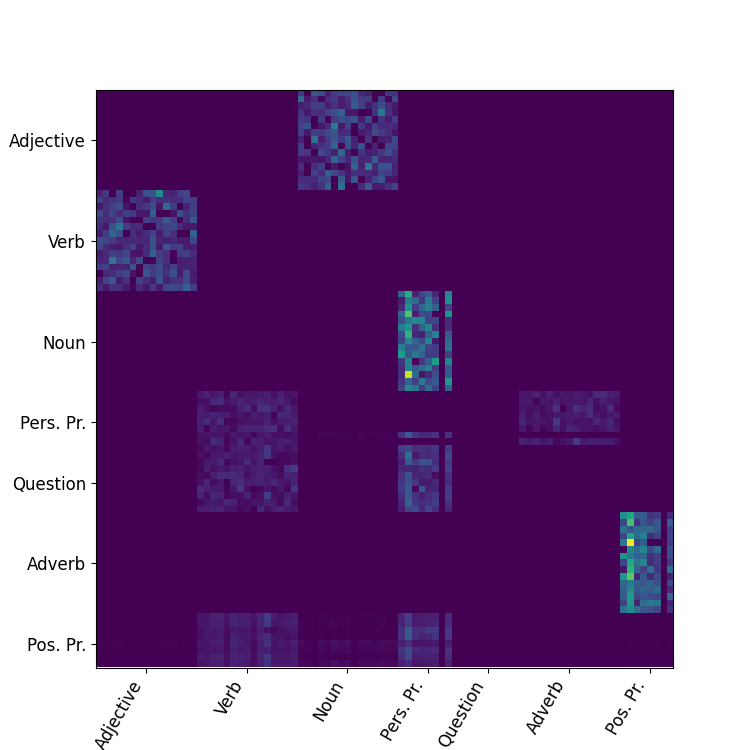
\includegraphics[height=0.98\columnwidth]{Bilder/results_first_model/8Rules/plots/First Model + More Rules_100E_100BS_1L_1C/Transition_Probability_Matrix;_t=1,_DF=0.5.png}
			\end{figure}
            \begin{center}
                {\large Learned SR}
            \end{center}
		\end{column}
		% SPALTE 2
		\begin{column}{0.33\textwidth}
    			\begin{figure}
    				\centering
    					\includegraphics<2->[height=0.98\columnwidth]{Bilder/results_first_model/8Rules/plots/First Model + More Rules_100E_100BS_1L_1C/MDS_of_Transition_Probability_Matrix;_t=1,_DF=0.5.png}
    			\end{figure}
            \Os{2}{
                \begin{center}
                    {\large MDS plot}
                \end{center}
            }
		\end{column}
		% SPALTE 3
		\begin{column}{0.33\textwidth}
%			\vspace*{7mm}
			\begin{figure}
				\centering
					\includegraphics<3->[height=0.98\columnwidth]{Bilder/results_first_model/4Rules/plots/First Model + More Rules_100E_100BS_1L_1C/SR,_t=2,_DF=0.5.png}
			\end{figure}
        \Os{3}{
            \begin{center}
                {\large SR for $ t=2 $, less word classes}
            \end{center}
        }
		\end{column}
	\end{columns}
% --------------------------------------
\mynote{
\begin{itemize}
    \item[üü] Finally, I will present the results.
    \item[ü] Again, we'll begin talking about the First Model
	\item Works well because the SR performs best in these well defined scenarios
	\item[i] To avoid clutter only word classes are labeled, indeed one row corresponds to one word.
	\item The MDS plot shows clustered word classes, which also means learning was successful. Although not necessary for this type of model, it offers some visual feedback for configurations using a larger data set because their matrix can't be plotted
	\item LETZTES BILD: SR for t=2, it is possible to recognize the following states of a {\huge \texttt{question word}}, here they are {\huge \texttt{Personal Pronoun}} and {\huge \texttt{Verb}}
\end{itemize}
}
% SAINT MARTIN MEMMINGEN
\end{frame}

% === Results – Word to word models 1/2 ===================================

\begin{frame}
\frametitle{Results – Word to word models}
	\begin{itemize}
		\item<+-> Comparison with a ground truth/statistical assessment possible by a metric
	\end{itemize}
	\vspace*{-1.5cm}
	\begin{columns}
		% SPALTE 1
		\begin{column}{0.33\textwidth}
			\begin{figure}
				\centering
					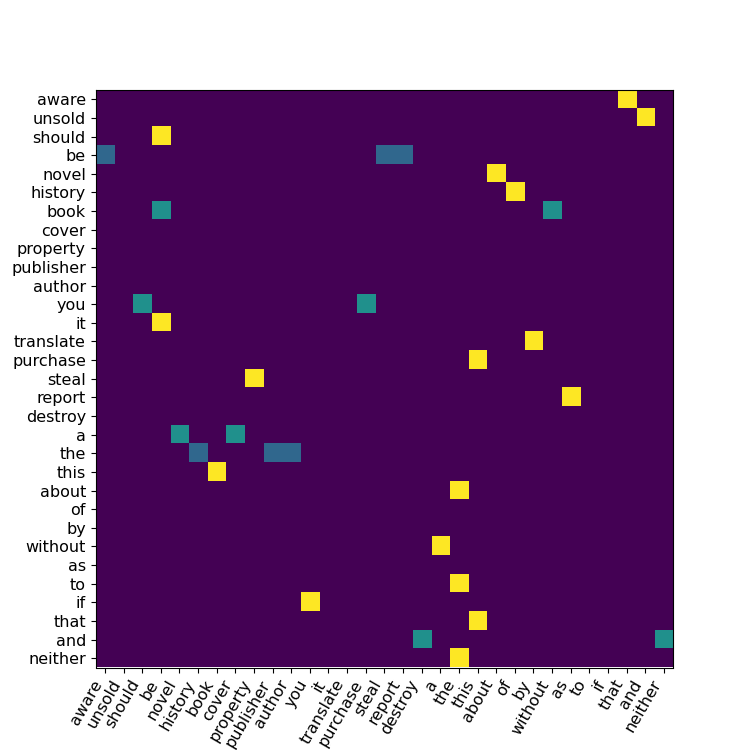
\includegraphics[height=1.1\columnwidth]{Bilder/BspW2W/plots/OHE_OHE_500E_100BS_1L_1C_5P_30T_J/J_5pages_30T_words.png}
			\end{figure}
			\begin{center}
				{\large Ground truth, Transition probability matrix}
			\end{center}
		\end{column}
		% SPALTE 2
		\begin{column}{0.33\textwidth}
			\begin{figure}
				\centering
					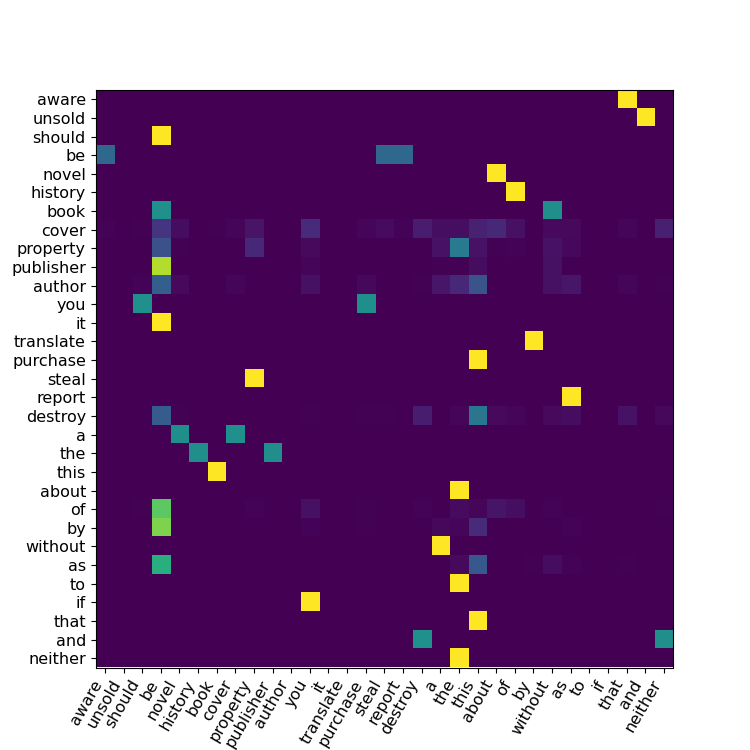
\includegraphics[height=1.1\columnwidth]{Bilder/BspW2W/plots/OHE_OHE_500E_100BS_1L_1C_5P_30T_J/Transition_Probability_Matrix;_t=1,_DF=0.5.png}
			\end{figure}
			\begin{center}
                {\large Learned transition probability matrix}
			\end{center}
		\end{column}
		% SPALTE 3
		\begin{column}{0.33\textwidth}
            \vspace*{8.5mm}
			\begin{figure}
				\centering
					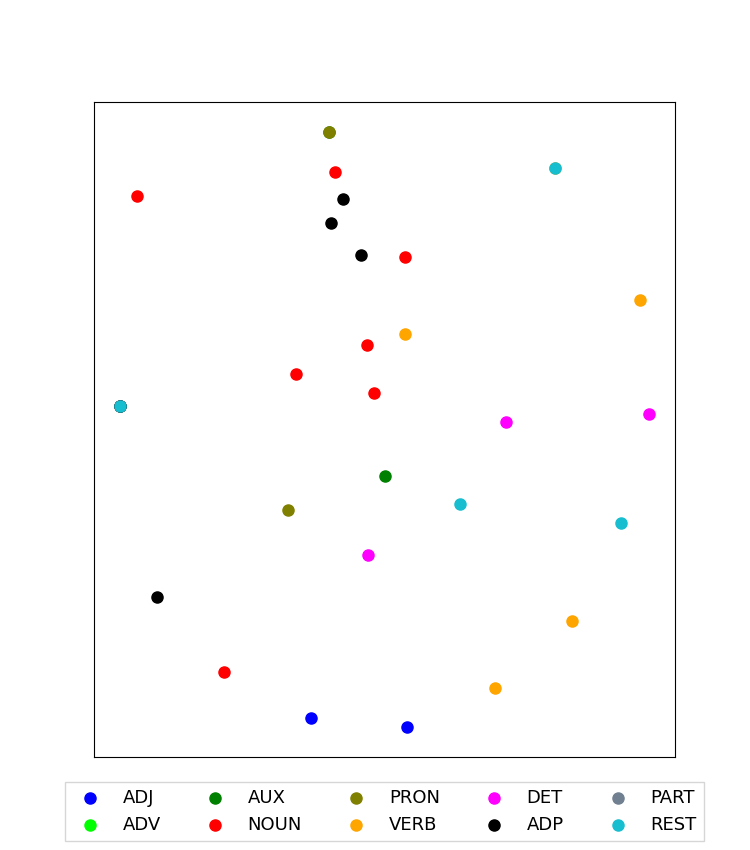
\includegraphics[height=1\columnwidth]{Bilder/BspW2W/plots/OHE_OHE_500E_100BS_1L_1C_5P_30T_J/MDS_of_Transition_Probability_Matrix;_t=1,_DF=0.5.png}
			\end{figure}
			\begin{center}
                {\large Learned MDS}
			\end{center}
		\end{column}
	\end{columns}
% --------------------------------------
\mynote{
\begin{itemize}
    \item[ü] word to word models show a different outcome.
    \item It is possible to compare the results to a ground truth/statistical assessment, hence the Metric $ d_A $ comes into play
	\item[i] On the left (LINKES BILD) is a ground truth depicted and next to it the predictions of the network. Although there is a resemblance visible it has to be assessed cautiously because a tiny data set was used for illustration purposes only to convey an intuition for the results and the procedure.
	\item[i] The MDS is displayed because matrices won't provide visual feedback anymore and as seen before sufficient learning is also visible in the cluster plot.
\end{itemize}
}
\end{frame}

% --- Results – Word to word modeles 2/2 -----------------------------------

\begin{frame}
	\frametitle{Results – Word to word models}
	\begin{itemize}
		\item<1-> It is possible to compare the results to a ground truth/statistical assessment $\Longrightarrow $ Metric $ d_A $
		\item<2-> Surprisingly \onehot{s} outperform word vectors i.e., word vectors are just bad
		\item<3-> German or english doesn't make that much of a difference
	\end{itemize}
	\begin{columns}
		% SPALTE 1
		\begin{column}{0.4\textwidth}
    \Os{1}{
			\vspace*{3mm}
			\begin{table}
%				\caption{Configurations with metric w.r.t. ground truth}
				\begin{tabular}{ll}
					\toprule
					Version					& Metric \\
					\midrule
					german, \onehot{} 		& $ 0.08 $	\\% 0.08200
					german, word vector		& $ 0.74 $	\\% 0.74139
					english, \onehot{}		& $ 0.10 $	\\% 0.10021
					english, word vector	& $ 0.78 $	\\% 0.77522
					\bottomrule
				\end{tabular}
			\end{table}
			\begin{center}
				{\large Configurations \& metric w.r.t. ground truth}
			\end{center}
            \vspace{3.2cm}\hspace*{5mm}\parbox{0.9\columnwidth}{{\normalsize \notsoimportant{If you want to know more about the metric, you can ask after the talk}}}
    }
		\end{column}
		% SPALTE 2
		\begin{column}{0.3\textwidth}
			\vspace*{-1cm}
			\begin{figure} % ohe de
				\centering
					\includegraphics<4->[height=0.55\textheight]{Bilder/W2W/OHE_OHE_5000E_100BS_1L_1C_200P_1500T_D/MDS_of_Transition_Probability_Matrix;_t=1,_DF=0.5.png}
			\end{figure}
    \Os{4}{
			\begin{center}
				{\large MDS of german, \onehot{}}
			\end{center}
    }
		\end{column}
		% SPALTE 3
		\begin{column}{0.3\textwidth}
			\vspace*{-1cm}
			\begin{figure} % w2v de
				\centering
					\includegraphics<4->[height=0.55\textheight]{Bilder/W2W/W2V_W2V_5000E_100BS_1L_1C_200P_1500T_D/MDS_of_Transition_Probability_Matrix;_t=1,_DF=0.5.png}
			\end{figure}
    \Os{4}{
			\begin{center}
				{\large MDS of german, word vectors}
			\end{center}
    }
		\end{column}
	\end{columns}
\mynote{
	\begin{itemize}
		\item In the table we find all four configurations comprising of \onehot{s} and word vector each ran with german and english.
        \begin{itemize}
            \item[i] The metric maps matrices close to $ 0 $ if the equal the ground truth and to $ 1 $ if not
        \end{itemize}
		\item Surprisingly \onehot{s} perform better than word vectors. Since they encode a word with more than two numbers, this was nothing to reckon with.
		\item We expected that english performs better than german due to the more static word order which was a fallacy
		\item In the image on the left is the MDS plot of the SR using \onehot{s} illustrated and on the right using word vectors. In both cases the hoped clusters didn't form and the configuration on the right seems to be omit a degenerated output at all. 
	\end{itemize}
}
\end{frame}

% === Results – Averaging models 1/3 ===================================

\begin{frame}{Results – Averaging models}
    \begin{itemize}
        \item<1-> Outcome of the plain vector models wasn't satisfying (as seen in the MDS plots), so averaging was established
    \item<2-> Results were indeed exploitable i.e., word class transition probabilities are partially reflected very accurately
    \end{itemize}
    \begin{columns}
        % SPALTE 1 ADP barplot
        \begin{column}{0.5\textwidth}
            \vspace*{-1cm}
            \begin{figure}
                \centering
                    \includegraphics<2->[width=0.66\textheight]{Bilder/Barplots/Avg_OHE_OHE_5000E_100BS_1L_1C_200P_1500T_D/Combined_Barplot_ADJ_F.png}
            \end{figure}
        \end{column}
        % SPALTE 2 ADJ barplot
        \begin{column}{0.5\textwidth}
            \vspace*{-1cm}
            \begin{figure}
                \centering
                    \includegraphics<2->[height=0.66\textheight]{Bilder/Barplots/Avg_OHE_OHE_5000E_100BS_1L_1C_200P_1500T_D/Combined_Barplot_ADP_S.png}
            \end{figure}
        \end{column}
    \end{columns}
% --------------------------------------
\mynote{
\begin{itemize}
    \item[ü] After all, coming to the Average Approach
    \item Because the outcome of the plain vector models wasn't satisfying (as illustarted in the MDS plot beforehand), an averaging approach was developed. Based on the predictions shown beforehand, transition probabilities between word classes were calculated
    \item The results are indeed exploitable especially using \onehot{s}. There, word class transitions are partially reflected very accurately as we can see in both bar plots
    \item[i] In both figures the learned probabilities and the ground truth probabilities are plotted, in blue and green respectively. The title is referring to the first word class, whereas the x axis shows the particular successor. Both diagrams show good accuracy for the word classes. 
\end{itemize}
}
\end{frame}

% --- Results – Averaging models 2/? -----------------------------------

\begin{frame}{Results – Averaging models}
    \begin{itemize}
        \item Matrices are $ 10 \times 10 $, so we display them
    \end{itemize}
    \vspace*{-1.5cm}
    \begin{columns}
        % SPALTE 1
        \begin{column}{0.33\textwidth}
            \begin{figure}
                \centering
                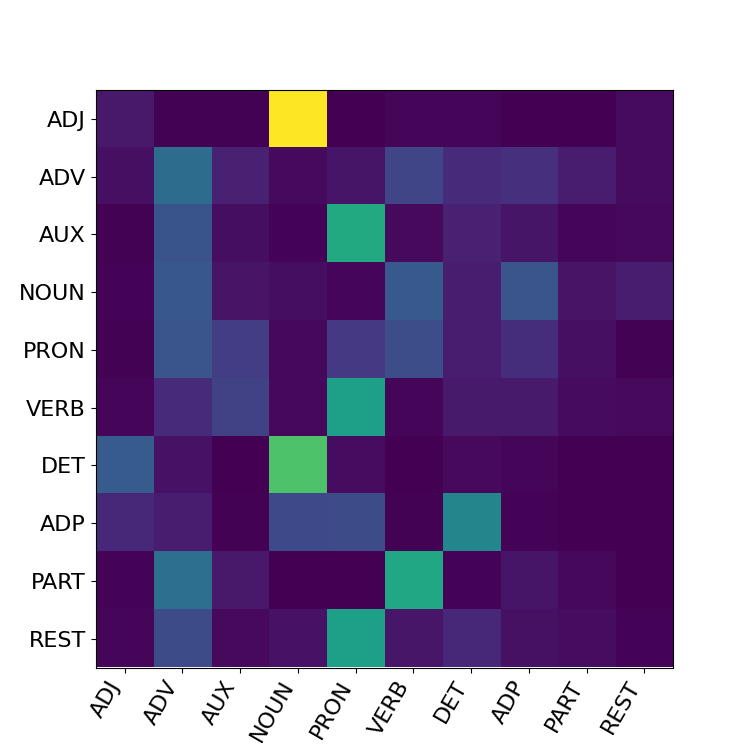
\includegraphics[width=1.1\columnwidth]{Bilder/average_models/ground_truths/D_200pages_1500T_tags.png}
            \end{figure}
            \begin{center}
                {\large ground truth (german)}
            \end{center}
        \end{column}
        % SPALTE 2
        \begin{column}{0.33\textwidth}
            \begin{figure}
                \centering
                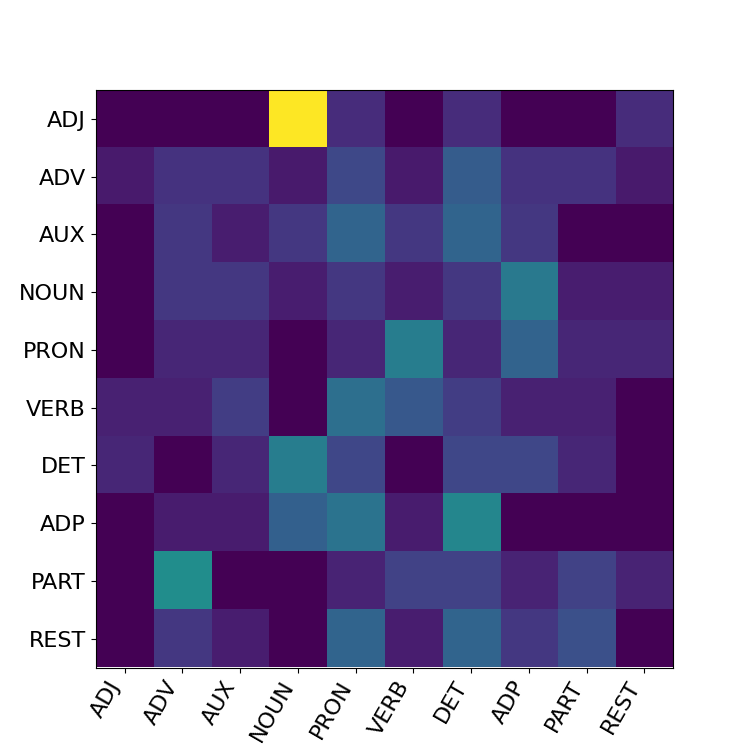
\includegraphics[width=1.1\columnwidth]{Bilder/average_models/Avg_OHE_OHE_5000E_100BS_1L_1C_200P_1500T_D/Transition_Probability_Matrix;_t=1,_DF=0.5.png}
            \end{figure}
            \begin{center}
                {\large german, \onehot{}} %:\\$ \mu = 7.3$, $ \sigma = 2.0 $
            \end{center}
        \end{column}
        % SPALTE 3
        \begin{column}{0.33\textwidth}
            \begin{figure}
                \centering
                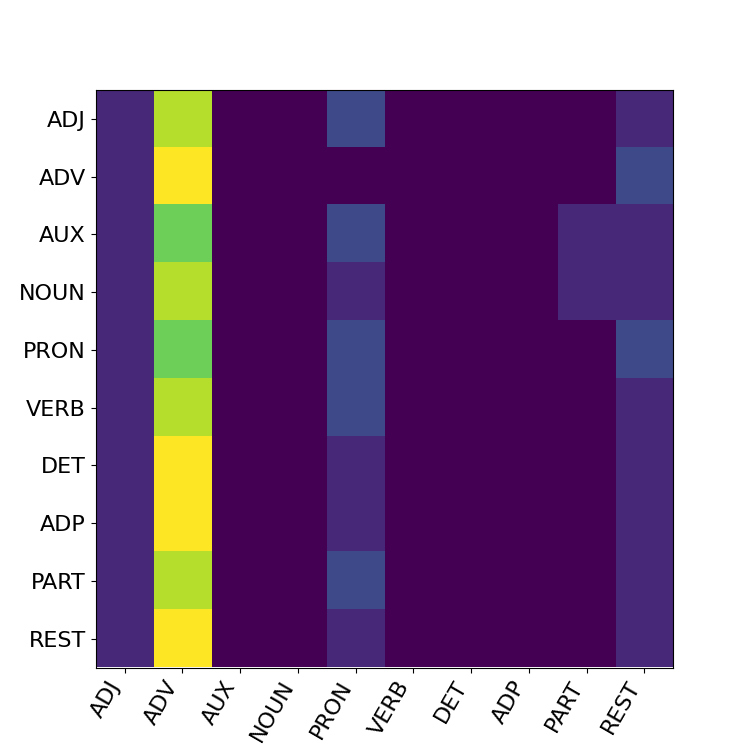
\includegraphics[width=1.1\columnwidth]{Bilder/average_models/Avg_W2V_W2V_5000E_100BS_1L_1C_200P_1500T_D/Transition_Probability_Matrix;_t=1,_DF=0.5.png}
            \end{figure}
            \begin{center}
                {\large german, word vector} %:\\$ \mu = 14.0$, $ \sigma = 2.1 $
            \end{center}
        \end{column}
    \end{columns}
% --------------------------------------
\mynote{
\begin{itemize}
    \item Matrices are $ 10 \times 10 $, so we display them
    \item[i] On the left there is the ground truth of the book illustrated, in the middle a \onehot{} model and on the right the word vector equivalent. The latter shows no learning at all, whereas similarities to the ground truth are recognizable in the middle.
    \item[i] The picture is similar for the english book
\end{itemize}
}
\end{frame}


% --- Results – Averaging models 2/3 -----------------------------------

\begin{frame}{Results – Averaging models}
    \begin{itemize}
        \item<+-> Accuracy of these models is measured by mean and standard deviation:
    \end{itemize}
    \begin{table}
        \centering
%        \caption{Averaged means of the difference between prediction and ground truth. As expected, the word vector versions have higher scores than the \onehot{} counterpart. These values can't be used for a comparison with \tabref{\ref{tab: text model versions and metrics}} because the underlying metrics are different.}
        \begin{tabular}{lrc}
            \toprule
            Version					& Mean $ \mu $		& Standard deviation $ \sigma $ \\
            \midrule
            german, \onehot{} 		& $ 7.3 $	& $ 2.0 $ \\% 0.08200
            german, word vector		& $ 14.0 $	& $ 2.1 $ \\% 0.74139
            english, \onehot{}		& $ 8.1 $	& $ 3.3 $ \\% 0.10021
            english, word vector	& $ 10.2 $	& $ 3.6 $ \\% 0.77522
            \bottomrule
        \end{tabular}
        \label{tab: avg model versions and metrics}
    \end{table}
    \hfill\notsoimportant{Mean and standard deviation in $ 10^{-2} $}
    \begin{itemize}
%        \item<+-> Again \onehot{s} outperform word vectors
        \item<+-> Sadly, the outcome of word vector models is quite bad again % (word vectors might be closer to real input signals of the hippocampus)
        \item<+-> But the \onehot{s} seem to grasp the grammatical structure (bar and matrix plot)
    \end{itemize}
% --------------------------------------
\mynote{
\begin{itemize}
    \item The accuracy of these models is measured by mean and standard deviation 	
    \item Sadly, the outcome of word vector models is not worth mentioning it again. This is in particular unsatisfactory because word vectors might be closer to real signals.
    \item But \onehot{} approaches seem to grasp the grammatical structure, which is justified by the bar and matrix plots   
    \item[x] FALLS JEMAND FRAGT Anderes Maß, es hier explizit die verschiedenen Zeilen mit der Ground truth verglichen wurden, Außerdem hat man weniger Spalten bzw. Zustände im Allgemeinen vorliegen, sodass man bspw. mit der Angabe der Standardabweichung auch etwas anfangen kann
    \item[x] FALLS JEMAND FRAGT
    \begin{itemize}
        \item[x] „Mean“ bedeutet: GT - SR, then row-wise mean, finally mean of means
        \item[x] „Std. deviation“ GT - SR, then row-wise std. dev., finally std. dev of std. devs.
    \end{itemize}
\end{itemize}
}
\end{frame}